\chapter{4541 Serial Bus Controller}

\newcolumntype{Y}[1]{%
  >{\small\raggedright\everypar{\hangindent=1em}\arraybackslash}p{#1}%
}

\section{Overview}

The 4541 is a Commodore{\texttrademark} serial peripheral bus compatible
bus controller, that greatly reduces the effort required to
communicate with devices on this bus.

\section{Features of the 4541}

\subsection{Supports Enhanced Serial Protocol Variants}

The 4541 supports the
JiffyDOS{\texttrademark} extensions to this protocol, that allow data
transfers approximately 10$\times$ faster than using the original
protocol. It is also expected that a future revision of the 4541 will
support Commodore's fast serial protocol, that is present in the 1571
and 1581 disk drives. 

\subsection{Interrupt Enabled Processor Offload}

The 4541 performs serial communications independent of the
microprocessor. Together with an IRQ functionality, this allows
software to continue on other tasks while serial peripheral
communications occurs, requiring only to be briefly interrupted when
the next event on the serial peripheral bus occurs.

\subsection{Processor Speed Independence}

A major advantage of the 4541, is that it also handles all timing
requirements of communications on this bus, allowing the bus to be
driven by a processor that can run at different speeds, without having
to modify the the bus controller software.

\subsection{Co-Existence through Open-Collector Logic}

Because the 4541 uses open-collector
logic, it can be used in parallel with existing software-based
implementations of the bus protocol, ensuring compatibility with
existing software.  It is installed in this configuration in the
MEGA65, allowing the legacy software-based serial peripheral
communications software that controls the serial peripheral bus to
continue to be used unmodified. 

\section{Theory of Operation}

The 4541 presents a quite simple interface: You issue commands, wait
for a response, and retrieve any data that the command
retrieved.  Some commands also require a data byte, which is provided
by a dedicated register.  There is also a device info register, that lets you see
what the 4541 believes about the current status of the most recently
requested device, including whether it is present, and whether it
supports either or both of the JiffyDOS{\texttrademark} or
Commodore{\textrademark} 128 extensions to the standard protocol.

So, for example, to release the Attention line, you can simply write
the appropriate command byte value (65 = \$41) to the command register
at \$D698, and then check for the completion status in the status
register at \$D697, as shown in the following example written in
BASIC65:

\begin{screencode}
  10 POKE $D698,$41
  20 IF ( PEEK($D697) AND $20 ) = $00 GOTO 20
  30 PRINT "DONE"
\end{screencode}

The 4541 implements a set of commands that map very closely to the
KERNAL calls that are used to control the IEC bus on the C64 and
related computers.  In most cases, there is a single corresponding
command for the 4541, although in a few cases, you may need to issue
two commands, as summarised in the following table:

\index{IEC Controller Commands}
\begin{center}
    \setlength{\def\arraystretch{1.5}\tabcolsep}{6pt}
    \begin{longtable}{|c|L{8cm}|}
        \hline
        \textbf{KERNAL Call} & \textbf{Meaning and Equivalent 4541 Command(s)}\\
        \hline
        \endhead
        \$FF93 LSTNSA & Send LISTEN secondary address.  \\
         & 4541 Equivalent: Data = Binary OR of \$60 and the desired
        secondary address.  Command \$30. Then Command \$41 to release
        the Attention line. \\
        \hline
        \$FF96 TALKSA & Sent TALK secondary address.  \\
         & 4541 Equivalent: Data = Binary OR of \$60 and the desired
        secondary address.  Command \$30. Then Command \$41 to release
        the Attention line. \\
        \hline
        \$FFA5 IECIN & Receive a byte from the serial peripheral bus.  \\
         & 4541 Equivalent : Command \$32. Received byte is available
        in the data register on completion.  \\
        \hline
        \$FFA8 IECOUT & Send a byte to the serial peripheral bus.  \\
         & 4541 Equivalent : Data = the byte to send. Command \$31 (or \$30 if the byte is to
        be sent under Attention). \\
        \hline
        \$FFA8 UNTALK  & Send UNTALK command to serial peripheral bus.  \\
        & 4541 Equivalent : Data = \$5F. Command \$30. \\    
        \hline
        \$FFAB UNLISTN  & Send UNLISTEN command to serial peripheral bus.  \\
        & 4541 Equivalent : Data = \$3F. Command \$30. \\    
        \hline
        \$FFB1 LISTEN  & Send LISTEN command to the serial peripheral bus.  \\
        & 4541 Equivalent : Data = \$20 plus the device number. Command \$30. \\    
        \hline
        \$FFB4 TALK  & Send TALK command to the serial peripheral bus.  \\
        & 4541 Equivalent : Data = \$40 plus the device number. Command \$30. \\    
        \hline
        \$FFB7 READST & Read the status of the serial peripheral bus.  \\
        & 4541 Equivalent : Read the status bits from \$D698. For
        convenience, the
        upper bits of this status byte have the same layout as used in
        the KERNAL. \\    
        \hline
    \end{longtable}
\end{center}

The 4541 is very obedient: If you ask it to do something new, it
will start doing that immediately, even if it was in the middle of
doing something else -- even if it was half-way through sending a byte
of data to the serial peripheral bus!  

You should therefore always wait until the IRQREADY bit in \$D697 is
set before issuing each command, or reading the status bits, to make
sure that the controller has finished whatever it was last asked to
do.

\section{Examples}

\subsection{Reading the DOS channel status}

The following BASIC65 program can be used to talk to a device
connected to the serial peripheral bus. Note that because it uses the
4541, and not the C65/MEGA65 CBDOS, it ignores the presence of the
internal 3.5'' disk drive, because that drive is not connected to the
serial peripheral bus.

\begin{screencode}
10 REM ABORT ANY EXISTING 4541 COMMAND IN PROGRESS
20 POKE $D698,$00
30 REM RESET THE SERIAL PERIPHERAL BUS BY PULLING
40 REM THE RESET PIN LOW FOR 1 SECOND
50 POKE $D698,$72 : SLEEP 1 : POKE $D698,$52
60 REM GIVE CONNECTED DEVICES TIME TO GET READY AFTER RESET
70 SLEEP 2: REM THE 1541 TAKES QUITE A WHILE TO RESET!
80 REM SELECT THE DEVICE NUMBER TO TALK TO
90 D = 8
100 PRINT"DEVICE"; D; "TALK"
110 POKE $D699,$40 + D : POKE $D698,$30 : GOSUB 1000
120 PRINT "SECONDARY ADDRESS 15"
130 POKE $D699,$6F : POKE $D698,$30 : GOSUB 1000
140 PRINT"TURN AROUND TO LISTEN"
150 POKE $D698,$35 : GOSUB 1000
160 PRINT "READ DOS STATUS"
170 POKE $D698,$32 : GOSUB 1000
180 PRINT CHR$( PEEK($D699) );
190 CC = CC + 1 : IF CC < 200 GOTO 180
999 END
1000 REM WAIT FOR 4541 TO FINISH COMMAND
1010 S=PEEK($D697) : IF (S AND 32) = 32 GOTO 1020
1020 GOTO 1000
1030 IF S AND 128 THEN PRINT "DEVICE NOT PRESENT" : END
1040 RETURN
\end{screencode}

If you have a 1581 with a JiffyDOS{\texttrademark} ROM connected, this
program will display something like the following when run:

\begin{screencode}
READY.
RUN
DEVICE 8 TALK
SECONDARY ADDRESS 15
TURN AROUND TO LISTEN
READ DOS STATUS
73,(C) 1989 JIFFYDOS 6.0 1581,00,00
00, OK,00,00
00, OK,00,00
00, OK,00,00
...
00, OK,0
READY.
\end{screencode}

\section{Command Reference}

The following table lists the set of command codes suppoprted by the 4541.

\begin{center}
    \setlength{\def\arraystretch{1.5}\tabcolsep}{6pt}
    \begin{longtable}{|c|L{8cm}|}
        \hline
        \textbf{Command Byte} & \textbf{Action} \\
        \hline
        \endhead
        \multicolumn{2}{c}{\textbf{Abort Running Commands}} \\
        \hline
        \$00 & Abort any executing command. \\
        \hline
        \$01 & Reset controller state: Release ATN, CLK, DATA, SRQ and enable default protocol selection. \\
        \hline
        \multicolumn{2}{c}{\textbf{Bit-Bashing Commands}} \\
        \hline
        \$41 & Release Attention (ATN) line to 5V. \\
        \hline
        \$61 & Pull Attention (ATN) line to 0V. \\
        \hline
        \$43 & Release clock (CLK) line to 5V. \\
        \hline
        \$63 & Pull clock (CLK) line to 0V. \\
        \hline
        \$44 & Release data (DATA) line to 5V. \\
        \hline
        \$64 & Pull data (DATA) line to 0V. \\
        \hline
        \$53 & Release fast serial clock (SRQ) line to 5V. \\
        \hline
        \$73 & Pull fast serial clock (SRQ) line to 0V. \\
        \hline
        \$52 & Pull reset (RESET) line to 0V. \\
        \hline
        \$72 & Release reset (RESET) line to 5V. \\
        \hline
        \multicolumn{2}{c}{\textbf{Protocol Variant Control Commands}} \\
        \hline
        \$4A & Enable solicitation of JiffyDOS{\texttrademark}
        extension to the serial protocol. \\
        \hline
        \$6A & Disable solicitation of JiffyDOS{\texttrademark}
        extension to the serial protocol. \\
        \hline
        \$46 & Enable solicitation of Commodore{\texttrademark} 1571/1581
        fast serial extension to the serial protocol. \\
        \hline
        \$66 & Disable solicitation of Commodore{\texttrademark} 1571/1581
        fast serial extension to the serial protocol. \\
        \hline

        \multicolumn{2}{c}{\textbf{Serial Bus Protocol Commands}} \\
        \hline
        \$30 & Send byte in \$D699 under attention. Attention line is
        held at 0V at the end of the transaction. \\
        \hline
        \$31 & Send bye in \$D699 without attention. The attention
        line is released, if it was previously asserted. \\
        \hline
        \$32 & Receive a byte from the peripheral serial bus. There
        must be a previously activated talker. The received byte is
        stored in \$D699. \\
        \hline
        \$33 & RESERVED \\
        \hline
        \$34 & Send a byte and indicate EOI. Attention is released
        prior to transmission, if was asserted. \\
        \hline
        \$35 & Turn around from talker to listener. \\
        \hline

        \multicolumn{2}{c}{\textbf{Protocol Timing Commands}} \\
        \hline
        \$80 & Reset protocol timing to defaults. \\ \hline
        \$81 & Set T\textsubscript{R} delay (1 -- 255 microseconds). Old value can be
        read from \$D699. \\ \hline
        \$82 & Set T\textsubscript{TK} delay (1 -- 255 microseconds). Old value can
        be read from \$D699. \\ \hline
        \$83 & Set T\textsubscript{DC} timeout (1 -- 255 milliseconds). Old value
        can be read from \$D699. \\ \hline        
        \$84 & Set T\textsubscript{BB} delay (1 -- 255 microseconds). Old value
        can be read from \$D699. \\ \hline        
        \$85 & Set T\textsubscript{HA} delay (1 -- 255 microseconds). Old value
        can be read from \$D699. \\ \hline        
        \$86 & Set T\textsubscript{ST} delay (1 -- 255 microseconds). Old value
        can be read from \$D699. \\ \hline        
        \$87 & Set T\textsubscript{VT} delay (1 -- 255 microseconds). Old value
        can be read from \$D699. \\ \hline        
        \$88 & Set T\textsubscript{AL} delay (1 -- 255 microseconds). Old value
        can be read from \$D699. \\ \hline        
        \$89 & Set T\textsubscript{AC} delay (1 -- 255 microseconds). Old value
        can be read from \$D699. \\ \hline        
        \$8A & Set T\textsubscript{AT} delay (1 -- 255 milliseconds). Old value
        can be read from \$D699. \\ \hline        
        \$8B & Set T\textsubscript{H} delay (1 -- 255 milliseconds). Old value
        can be read from \$D699. {\em This value currently has no
          effect, as the 4541 allows truly infinite data-hold off by a
          listener, except for bytes sent under attention, where
          T\textsubscript{HA} is used instead.}\\ \hline        
        \$8C & Set T\textsubscript{NE} delay (1 -- 255 microseconds). Old value
        can be read from \$D699. \\ \hline        
        \$8D & Set T\textsubscript{F} delay (4 -- 1020 microseconds). Old value
        can be read from \$D699, scaled by 4. \\ \hline        
        \$8E & Set T\textsubscript{YE} delay (1 -- 255 microseconds). Old value
        can be read from \$D699. \\ \hline        
        \$8F & Set T\textsubscript{EI} delay (1 -- 255 microseconds). Old value
        can be read from \$D699. \\ \hline        
        \$90 & Set T\textsubscript{AR} delay (1 -- 255 microseconds). Old value
        can be read from \$D699. \\ \hline        
        \$91 & Set T\textsubscript{JT} delay (4 -- 1020 microseconds). Old value
        can be read from \$D699, scaled by 4. \\ \hline        
        \$92 & Set T\textsubscript{J0} delay (1 -- 255 microseconds). Old value
        can be read from \$D699. \\ \hline        
        \$93 & Set T\textsubscript{J1} delay (1 -- 255 microseconds). Old value
        can be read from \$D699. \\ \hline        
        \$94 & Set T\textsubscript{J2} delay (1 -- 255 microseconds). Old value
        can be read from \$D699. \\ \hline        
        \$95 & Set T\textsubscript{J3} delay (1 -- 255 microseconds). Old value
        can be read from \$D699. \\ \hline        
        \$96 & Set T\textsubscript{J4} delay (1 -- 255 microseconds). Old value
        can be read from \$D699. \\ \hline        
        \$97 & Set T\textsubscript{J5} delay (1 -- 255 microseconds). Old value
        can be read from \$D699. \\ \hline        
        \$98 & Set T\textsubscript{J6} delay (1 -- 255 microseconds). Old value
        can be read from \$D699. \\ \hline        
        \$99 & Set T\textsubscript{J7} delay (1 -- 255 microseconds). Old value
        can be read from \$D699. \\ \hline        
        \$9A & Set T\textsubscript{J8} delay (1 -- 255 microseconds). Old value
        can be read from \$D699. \\ \hline        
        \$9B & Set T\textsubscript{J9} delay (1 -- 255 microseconds). Old value
        can be read from \$D699. \\ \hline        
        \$9C & Set T\textsubscript{J10} delay (1 -- 255 microseconds). Old value
        can be read from \$D699. \\ \hline        
        \$9D & Set T\textsubscript{J11} delay (1 -- 255 microseconds). Old value
        can be read from \$D699. \\ \hline        
        \$9E & Set T\textsubscript{JR} delay (1 -- 255 microseconds). Old value
        can be read from \$D699. \\ \hline        
        \$9F & Set T\textsubscript{FS} delay (1 -- 255 microseconds). Old value
        can be read from \$D699. \\ \hline        
        \$A0 & Set T\textsubscript{FF} delay (1 -- 255 microseconds). Old value
        can be read from \$D699. \\ \hline        
        \$A1 & Set T\textsubscript{PULLUP} delay (1 -- 255 microseconds). Old value
        can be read from \$D699. \\ \hline        
        \$A2 & Set T\textsubscript{JD} delay (4 -- 1020 microseconds). Old value
        can be read from \$D699, scaled by 4. \\ \hline        
        
        \multicolumn{2}{c}{\textbf{Diagnostic Commands}} \\
        \hline
        \$D0 & Trigger optional integrated data logger, if enabled. \\
        \hline
        \$D1 & Begin transmitting a 1KHz pulse train on the CLK and
        DATA lines. Continues until aborted by another command. \\
        \hline
    \end{longtable}
\end{center}


\section{Register Table}

The 4541 has the following registers:

\input{regtable_AUTOIEC.MEGA65}

\section{Serial Bus Timing}

This section describes the timing requirements primarily from the
perspective of a bus controller. If you are designing serial bus
peripherals, please take care to carefully understand how these time
requirements affect peripherals: The 


\subsection{Send Byte Under Attention}

When the controller wishes to get the attention of one or more
peripherals on the bus, it uses the attention (ATN) line to indicate
this: It pulls it low to 0V, and then sends one or more bytes that
will be received by all devices on the bus.

The SRQ line is not active in this transaction.

To summarise:

\begin{enumerate}
\item The controller pulls the ATN to 0V and releases the CLK, DATA
  and SRQ lines if it was holding any of them at 0V.
\item All peripherals on the bus as they notice the ATN line at 0V
  begin to indicate this by pulling the DATA line to 0V.
  The controller can't tell how many, or whether all the devices
  on the bus have responded: Rather, it can only tell that at least
  one device has.
\item If no device responds, DATA stays at 5V, because no one is
  pulling it down, and the
  controller will indicate a DEVICE NOT PRESENT error.
\item While the controller is waiting for devices to respond, it
  also pulls the CLK line to 0V, typically a short time after
  pulling the ATN line to 0V.
\item After the controller has waited a while, typically 1
  millisecond, it assumes that all peripherals who are going to
  answer the ATN request have.
\item Next, the controller releasing the CLK line to 5V to indicate
  that it wants to send a byte of data on the bus. This is the start
  of the transmission of a byte under ATN. All of the previous steps
  have had the purpose of establishing the ATN communications.
\item The controller now waits for all devices to indicate
  their readiness to receive a byte by releasing the DATA line
  back to 5V. Because the bus is open-collector, if even a
  single device is not ready, it will be able to keep pulling
  the DATA line down to 0V, causing the controller to wait.
  If this takes too long, the controller may give up and
  indicate a timeout condition.
\item Once the last device has indicate it is ready to receive data,
  the controller waits a little longer, to make sure that all of the
  devices are able to do their final preparations to receive a
  byte. This doesn't take very long.
\item After that delay, the controller begins sending the 8 bits of
  data, beginning with the least significant bit (LSB), that is bit
  0. For each bit, it first brinks the CLK line low to indicate that
  data is being loaded onto the bus, pulls the DATA line to 0V if it
  wants to send a 0 bit, or lets it float to 5V if it wants to send
  a 1 bit, and then releases the CLK line back to 5V, and holds it
  there for a while.  The timing of this process is critical: If the
  CLK is low or high for too short a period of time, the peripherals
  will get confused, and possibly miss one or more bits, resulting
  in general chaos on the bus.
\item After the controller has sent the last bit, it holds the CLK
  line low, and releases the DATA line. It expects one or more
  peripherals to pull the DATA line to 0V within a short time to
  acknowledge reception of the byte. If this does not occur, the
  controller may report a timeout or DEVICE NOT PRESENT error.
\item At the conclusion of this, the controller is holding the
  CLK line at 0V, and the peripheral(s) are holding the DATA
  line at 0V. This combination serves to tell each other that
  the controller is not yet wanting to send the next byte, and
  that the peripheral(s) are not yet ready to receive the next
  byte.
\item If the controller wishes to send more bytes under
  attention, it will repeat this process from the step where
  it released the CLK line to 5V.
\item Alternatively, if it was the last byte to be sent
  under this attention request, the controller waits a short
  time, and then releases the ATN line.
\end{enumerate}

\begin{center}
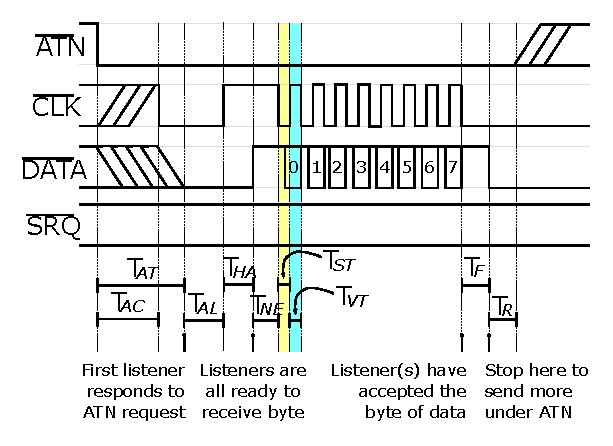
\includegraphics{images/IEC-Timing-Diagrams/IEC-Timing-Diagram-ATN-Send-Byte}
\end{center}

\begin{center}
    \setlength{\def\arraystretch{1.5}\tabcolsep}{6pt}
    \begin{longtable}{|L{0.6cm}|c|c|c|c|L{6cm}|}
      \hline
        \multicolumn{2}{|c|}{\textbf{Symbol}} & \textbf{Min} & \textbf{4541} & \textbf{Max} & \textbf{Description} \\
        \hline
        \endhead
        \multicolumn{2}{|c|}{T\textsubscript{AT}} & --  & 1000 & $\infty$ &
        Device attention response timeout. {\em A device must
          respond to the ATN request within this time. If not device
          responds within this time, a DEVICE NOT PRESENT error will
          result. Peripherals should therefore conform to the 1,000
          microsecond typical value.} \\
        \hline
        \multicolumn{2}{|c|}{T\textsubscript{AC}} & --  & 20 & $\infty$? &
        Time between pulling ATN low, before CLK is also pulled low. \\
        \hline
        \multicolumn{2}{|c|}{T\textsubscript{AL}} & --  & 1000 & $\infty$? &
        Time between first device responds to ATN and the controller releases CLK
        to 5V. \\
        \hline
        \multicolumn{2}{|c|}{T\textsubscript{HA}} & -- & 64 ms & $\infty$ & Listener
        hold-off. {\em The protocol allows a listener can hold of for any desired period of
          time, or for no time at all. The 4541 does not allow this
          during ATN requests.} \\
        \hline
        \multicolumn{2}{|c|}{T\textsubscript{NE}} & --  & 40 & 200 &
        Non-EOI timing-channel response to Ready For Data. {\em If
          this interval is too long, the byte will be interpreted as
          an EOI byte, and the peripherals will require an EOI
          response (see T\textsubscript{EI}).} \\
        \hline
        \multicolumn{2}{|c|}{T\textsubscript{ST}} & 20*  & 35 & $\infty$ &
        Data bit setup time. {\em Referred to as T\textsubscript{S} in
          the C64 Programmer's Reference Guide.}\\
        \hline
        \multicolumn{2}{|c|}{T\textsubscript{VT}} & 20*  & 35 & $\infty$ &
        Data bit valid hold time. {\em Referred to as
          T\textsubscript{V} in the C64 Programmer's Reference Guide.} \\
        \hline
        \multicolumn{2}{|c|}{T\textsubscript{F}} & --  & 1000 & 1000 &
        Frame handshake (acknowledge) timeout. \\
        \hline
        \multicolumn{2}{|c|}{T\textsubscript{R}} & 20  & 200 & $\infty$ &
        Time between receiving end of frame acknowledgement and
        releasing the ATN line to 5V. \\
        \hline
        \multicolumn{6}{l}{\em All time units are in micro seconds, unless
          otherwise indicated.} \\
        \multicolumn{6}{Y{10cm}}{*{}
          The Commodore{\texttrademark} 64 Programmer's Reference
          Guide suggests that T\textsubscript{S} and
          T\textsubscript{V} each have a minimum duration of 20 micro seconds.
          Our investigations suggest that when communicating with a
          1541, that safe values for 
          T\textsubscript{ST} and T\textsubscript{VT} are closer to 70
          micro seconds.
        }
          \\
        
    \end{longtable}
\end{center}

\subsection{JiffyDOS{\texttrademark} Protocol Solicitation}

If support for the JiffyDOS{\texttrademark} protocol extension is
enabled, the 4541 will solicit this during the transmission of TALK
and LISTEN commands only. That is, when sending a byte under attention
that is in the range \$20 -- \$5F.

The SRQ line is not active in this transaction.

To summarise:

\begin{enumerate}
  \item The transmission of the byte occurs normally, until the
    T\textsubscript{ST} period just before the last bit (bit 7) of the
    byte.
  \item Instead of waiting T\textsubscript{ST}, the controller must
    instead wait for a much longer period, typically 300
    microseconds, so that the listener will recognise that it is
    being asked if it supports the JiffyDOS{\textrademark}
    protocol. The controller also releases the DATA line to 5V.
  \item If the listener supports the JiffyDOS{\texttrademark} protocol,
    it pulls DATA to 0V when it observes that the CLK line has been
    held low for the longer period.
  \item After the listener has held DATA at 0V long enough for it
    to be sure the controller has had the chance to notice, it
    releases the DATA line to 5V. The device will now use the
    JiffyDOS{\texttrademark} for the requested TALK or LISTEN session.
  \item The controller notes if the DATA line was pulled to 0V, and if
    so, records that the listener has selected the
    JiffyDOS{\texttrademark} protocol, and will use this protocol for the
    requested TALK or LISTEN session.
  \item The controller now sends the final bit of the byte.
  \item The controller ensures that the data bit value is visible on
    DATA before asserting CLK, typically 1 -- 4 microseconds.
  \item The controller releases the CLK line to 5V to indicate to
    the listener that the final data bit is ready.
  \item The remainder of the byte transfers as normal.
\end{enumerate}

\begin{center}
\includegraphics{images/IEC-Timing-Diagrams/IEC-Timing-Diagram-ATN-JD-Solicit}
\end{center}

\begin{center}
    \setlength{\def\arraystretch{1.5}\tabcolsep}{6pt}
    \begin{longtable}{|L{0.6cm}|c|c|c|c|L{6cm}|}
      \hline
        \multicolumn{2}{|c|}{\textbf{Symbol}} & \textbf{Min} & \textbf{4541} & \textbf{Max} & \textbf{Description} \\
        \hline
        \endhead
        \multicolumn{2}{|c|}{T\textsubscript{JD}} & 320  & 320 & $\infty$ &
        Time that CLK is held at 0V between the two final bits of the
        byte to provide the side-channel indication that the
        controller wishes to use the JiffyDOS{\texttrademark} protocol extension.
        \\
        \hline
        \multicolumn{2}{|c|}{T\textsubscript{IJ}} & 100  & -- & 295 &
        Time before the listener accepts and begins to acknowledge the
        selection of the JiffyDOS{\texttrademark} protocol extension.
        \\
        \hline
        \multicolumn{2}{|c|}{T\textsubscript{IJ}} & 4/100*  & -- & 200 &
        The duration that the listener holds the DATA line low to
        acknowledge the 
        selection of the JiffyDOS{\texttrademark} protocol extension.
        \\
        \hline
        \multicolumn{6}{l}{\em All other timing values are identical to the sending a byte
          under attention case.}
          \\
        \multicolumn{6}{l}{\em All time units are in micro seconds, unless
          otherwise indicated.} \\
        \multicolumn{6}{Y{10cm}}{*{}
          The 4541 can detect pulse-widths as narrow as 4
          microseconds. However, software implementations of the
          protocol will require a larger value. JiffyDOS\texttrademark
          uses 100 microseconds.
        }

        
    \end{longtable}
\end{center}

\subsection{JiffyDOS{\texttrademark} Send from Controller to Peripheral}

Unlike the standard serial protocol, the JiffyDOS{\texttrademark} protocol uses
different protocols for sending and receiving. This is necessary on software
imeplementations to obtain the maximum speed, because the serial peripheral
lines are mapped to different register bits, and part of the magic of
the JiffyDOS{\texttrademark} protocol is how it cleverly manipulates
the received bits to reconstruct the complete byte in the least
possible time, and similarly when transmitting.

The result is quite amazing: JiffyDOS{\texttrademark} can send a byte
in approximately the same time it takes the original protocol to send
a bit!

Note that the JiffyDOS{\texttrademark} protocol transmits data bits with the opposite polarity
to the standard protocol, that is a 1 bit is indicated by 0V, while a
0 bit is indicated by 5V.

The SRQ line is not active in this transaction.

In summary,

\begin{enumerate}
\item Depending on the state of the controller when it begins
  transmitting, it may be holding the CLK line at 0V. If so it
  releases it immediately.
\item Next, after some arbitrary time, the peripheral indicates
  it's readiness to receive a byte from the controller by
  releasing the DATA line to 5V.
\item The timing for the remainder of the byte transfer is now
  critical, because immediately following releasing DATA, the
  peripheral will start reading the CLK and DATA signals to
  transfer the byte.
\item The controller waits a few microseconds
  (T\textsubscript{J6}).
\item The controller sets CLK to 0V if data bit 4 is 1, else
  releases it to 5V.  The controller sets DATA to 0V if data
  bit 5 is 1, else releases it to 5V.
\item The controller waits a few microseconds
  (T\textsubscript{J7}).
\item The controller sets CLK to 0V if data bit 6 is 1, else
  releases it to 5V.  The controller sets DATA to 0V if data
  bit 7 is 1, else releases it to 5V.
\item The controller waits a few microseconds
  (T\textsubscript{J8}).
\item The controller sets CLK to 0V if data bit 3 is 1, else
  releases it to 5V.  The controller sets DATA to 0V if data
  bit 1 is 1, else releases it to 5V.
\item The controller waits a few microseconds
  (T\textsubscript{J9}).
\item The controller sets CLK to 0V if data bit 2 is 1, else
  releases it to 5V.  The controller sets DATA to 0V if data
  bit 0 is 1, else releases it to 5V.
\item The controller waits a few microseconds
  (T\textsubscript{J10}).
\item The controller pulls the DATA line to 0V. It also releases the
  CLK line to 5V, unless it wishes to indicate EOI, in which
  case it pulls the CLK line to 0V.
\item The controller waits a few microseconds, during which time the
  peripheral reads the EOI value, and then pulls DATA to 0V.
  (T\textsubscript{J11}).
\item The byte transfer is complete.
\end{enumerate}

Note when sending the first byte under the JiffyDOS{\texttrademark}
protocol, that the CLK signal may be at 0V.  The time between bytes
(T\textsubscript{JBB}) is not required (set to zero), because the
tight receive loop on the peripheral simply indicates when it is ready
to receive each next byte, which also contributes to it's high speed.

Note also that the timing below is based on when the signals should be
set. For software implementations, the latency of the necessary
processor instructions must be taken into account. This is not a
problem with the 4541, because it has a latency of less than 50ns.

\begin{center}
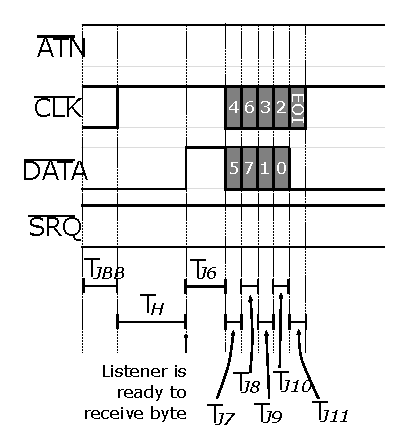
\includegraphics{images/IEC-Timing-Diagrams/IEC-Timing-Diagram-Send-Byte-JD}
\end{center}

\begin{center}
    \setlength{\def\arraystretch{1.5}\tabcolsep}{6pt}
    \begin{longtable}{|L{0.6cm}|c|c|c|c|L{6cm}|}
      \hline
        \multicolumn{2}{|c|}{\textbf{Symbol}} & \textbf{Min} & \textbf{4541} & \textbf{Max} & \textbf{Description} \\
        \hline
        \endhead
        \multicolumn{2}{|c|}{T\textsubscript{JBB}} & 0  & 0 & $\infty$ &
        Time between bytes.
        There is no minimum time between bytes with the 
        JiffyDOS{\texttrademark} protocol,
        provided T\textsubscript{J11} is sufficiently large, as that
        effectively hides the latency of the receive routine. \\
        \hline
        \multicolumn{2}{|c|}{T\textsubscript{J6}} & 10  & 10 & 10 &
        JiffyDOS{\texttrademark} transmit receiver setup time. \\
        \hline
        \multicolumn{2}{|c|}{T\textsubscript{J7}} & 13  & 13 & 13 &
        JiffyDOS{\texttrademark} transmit hold time, first di-bit. \\
        \hline
        \multicolumn{2}{|c|}{T\textsubscript{J8}} & 11  & 11 & 11 &
        JiffyDOS{\texttrademark} transmit hold time, second di-bit. \\
        \hline
        \multicolumn{2}{|c|}{T\textsubscript{J9}} & 11  & 11 & 11 &
        JiffyDOS{\texttrademark} transmit hold time, third di-bit. \\
        \hline
        \multicolumn{2}{|c|}{T\textsubscript{J10}} & 12  & 12 & 12 &
        JiffyDOS{\texttrademark} transmit hold time, fourth di-bit. \\
        \hline
        \multicolumn{2}{|c|}{T\textsubscript{J11}} & 28  & 28 & 28 &
        JiffyDOS{\texttrademark} transmit hold time, status bits. CLK
        carries the EOI notification, and DATA is set to 0V to
        indicate successful transmission. The receiver may indicate a
        frame error if DATA is observed to be 5V.  \\
        \hline
        \multicolumn{6}{l}{\em All other timing values are identical to the sending a byte
          under attention case.}
          \\
        \multicolumn{6}{l}{\em All time units are in micro seconds, unless
          otherwise indicated.} \\
        
    \end{longtable}
\end{center}

\subsection{JiffyDOS{\texttrademark} Controller Receive from Peripheral}

Unlike the standard serial protocol, the JiffyDOS{\texttrademark} protocol uses
different protocols for sending and receiving. This is necessary on software
imeplementations to obtain the maximum speed, because the serial peripheral
lines are mapped to different register bits, and part of the magic of
the JiffyDOS{\texttrademark} protocol is how it cleverly manipulates
the received bits to reconstruct the complete byte in the least
possible time, and similarly when transmitting.

The result is quite amazing: JiffyDOS{\texttrademark} can send a byte
in approximately the same time it takes the original protocol to send
a bit!

Unlike when transmitting via the JiffyDOS{\texttrademark} protocol
where the data bits are inverted, when receiving from a peripheral
speaking the JiffyDOS{\texttrademark} protocol, the bits are
represented naturally, i.e., with 1 = 5V and 0 = 0V.

The SRQ line is not active in this transaction.

To summarise:

\begin{enumerate}
\item The peripheral may wait an arbitrary period of time, before it
  has a byte to send to the controller. When it does, it releases CLK
  to 5V.
\item When the controller notices this, it releases DATA to 5V, and
  begins the critical timing section of the protocol.
\item The peripheral waits a short while. For peripherals using a
  software-implementation, i.e., all Commodore{\texttrademark}
  drives, the delay is a natural consequence of the processor
  instruction involved in commencing sending of the byte,
  similarly for the following steps.
\item The peripheral places the first di-bit of data on the CLK
  and DATA lines, and waits a short while.
\item The peripheral places the second di-bit of data on the CLK
  and DATA lines, and waits a short while.
\item The peripheral places the third di-bit of data on the CLK
  and DATA lines, and waits a short while.
\item The peripheral places the fourth di-bit of data on the CLK
  and DATA lines, and waits a short while.
\item The peripheral places the status bits for the byte onto
  the CLK and DATA lines, and waits a short while.
\item The controller pulls DATA to 0V to acknowledge receipt
  of the byte, and to prevent the peripheral from sending
  another byte before it is ready.
\item The peripheral pulls the CLK line to 0V if it does not
  have another byte ready to send immediately, lease it
  remains at 5V.
\end{enumerate}

The status bits have the following interpretation:

\begin{center}
    \setlength{\def\arraystretch{1.5}\tabcolsep}{6pt}
    \begin{longtable}{|c|c|L{6cm}|}
      \hline
        \textbf{CLK} & \textbf{DATA} & \textbf{Meaning} \\
        \hline
        \endhead
        0V & 0V & An error occurred. \\ 
        \hline
        0V & 5V & Byte received with EOI. \\
        \hline
        5V & 0V & Normal byte received (no EOI). \\
        \hline
        5V & 5V & An error occurred. \\
        \hline
    \end{longtable}
\end{center}

\begin{center}
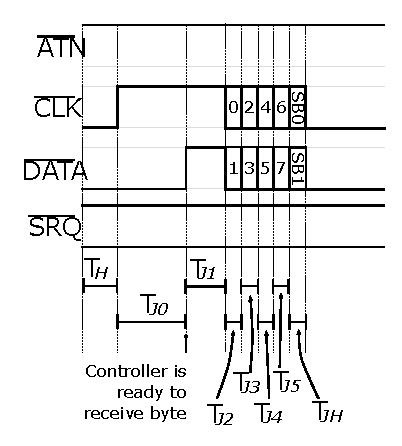
\includegraphics{images/IEC-Timing-Diagrams/IEC-Timing-Diagram-Receive-Byte-JD}
\end{center}

\begin{center}
    \setlength{\def\arraystretch{1.5}\tabcolsep}{6pt}
    \begin{longtable}{|L{0.6cm}|c|c|c|c|L{6cm}|}
      \hline
        \multicolumn{2}{|c|}{\textbf{Symbol}} & \textbf{Min} & \textbf{4541} & \textbf{Max} & \textbf{Description} \\
        \hline
        \endhead
        \multicolumn{2}{|c|}{T\textsubscript{JH}} & 10  & -- & $\infty$ & 
        Peripheral hold-off until it has data to send. \\
        \hline
        \multicolumn{2}{|c|}{T\textsubscript{J0}} & 0  & -- & $\infty$ &
        Controller hold-off until ready to receive a byte. \\
        \hline
        \multicolumn{2}{|c|}{T\textsubscript{J1}} & 37  & 37 & $\infty$ &
        The time is
        used by software implementations to prepare the byte for
        immediate transmission. \\
        \hline
        \multicolumn{2}{|c|}{T\textsubscript{J2}} & 14  & 14 & 14 &
        Send first di-bit of data \\
        \hline
        \multicolumn{2}{|c|}{T\textsubscript{J3}} & 10  & 10 & 10 &
        Send first di-bit of data \\
        \hline
        \multicolumn{2}{|c|}{T\textsubscript{J4}} & 11  & 11 & 11 &
        Send first di-bit of data \\
        \hline
        \multicolumn{2}{|c|}{T\textsubscript{J5}} & 11  & 11 & 11 &
        Send first di-bit of data \\
        \hline
        \multicolumn{2}{|c|}{T\textsubscript{JH}} & 13  & 13 & 13 &
        Send status bits \\
        \hline
        \multicolumn{6}{l}{\em All other timing values are identical to the sending a byte
          under attention case.}
          \\
        \multicolumn{6}{l}{\em All time units are in micro seconds, unless
          otherwise indicated.} \\
        
    \end{longtable}
\end{center}



\subsection{Talker to Listener Turn-Around}

When the bus controller is commanding a device to talk, it finished
the transmission with ATN asserted to 0V.  The controller is holding
the CLK line at 0V, and the device it was talking to is holding the
DATA line.  This situation needs to be reversed: The controller needs
to give up control of the bus, and hand it over to the device.

The SRQ line is not active in this transaction.

To summarise:

\begin{enumerate}
\item The controller waits long enough before releasing the
ATN line, to make sure that the peripheral(s) has finished acknowledging the
byte that was just sent to it under attention. This is the T\textsubscript{R} delay.
\item The controller releases the ATN line to 5V.
\item The controller waits a while. This is the T\textsubscript{TK} delay.
\item The controller releases the CLK line to 5V, and pulls the DATA
  line to 0V. From this point
  forward, the controller has relinquished control of the bus, and
  becomes a listener.
\item After some period of time, the peripheral that has been
  commanded to talk asserts the CLK line to 0V, and releases the DATA
  line, which remains at 0V, because the the controller is still
  pulling it down to 0V in preparation to be the listener.
  From this point
  in time, the peripheral has become the sole talker on the
  bus. The delay before the CLK line is pulled to 0V by the
  peripheral is the T\textsubscript{DC} timeout.
\item The peripheral waits a while, before it is allowed to
  begin talking. This is the T\textsubscript{DA} delay.
\end{enumerate}

Once this process is complete, the roles of the controller and
peripheral have reversed, with the peripheral now having the role of
talker, and the controller (and possibly other devices on the bus) of
listener.

\begin{center}
\includegraphics{images/IEC-Timing-Diagrams/IEC-Timing-Diagram-TurnAround}
\end{center}

\begin{center}
    \setlength{\def\arraystretch{1.5}\tabcolsep}{6pt}
    \begin{longtable}{|L{0.6cm}|c|c|c|c|L{6cm}|}
      \hline
        \multicolumn{2}{|c|}{\textbf{Symbol}} & \textbf{Min} & \textbf{4541} & \textbf{Max} & \textbf{Description} \\
        \hline
        \endhead
        \multicolumn{2}{|c|}{T\textsubscript{DA}} & 4/80* & -- & $\infty$ &
        Talk-Attention acknowledge hold duration. Controller holds CLK
        \\
        \hline
        \multicolumn{2}{|c|}{T\textsubscript{DC}} & 0 & 64 ms & $\infty$ & Talk-Attention acknowledge
        duration, i.e., the time a peripheral is permitted to take
        before becoming talker. {\em Can commence immediately when CLK is observed
        at 5V.}\\
        \hline
        \multicolumn{2}{|c|}{T\textsubscript{H}} & -- & N/A & $\infty$ & Listener
        hold-off. {\em Listener can hold of for any desired period of
          time, or for no time at all.} \\
        \hline
        \multicolumn{2}{|c|}{T\textsubscript{R}} & 0/20\^{} & 200 & -- & Frame to
        release of ATN. \\
        \hline
        \multicolumn{2}{|c|}{T\textsubscript{TK}} & 20 & 40 & 100 & Talk
        Attention Release. \\
        \hline
        \multicolumn{6}{l}{\em All time units are in micro seconds, unless
          otherwise indicated.} \\
        \multicolumn{6}{Y{10cm}}{* T\textsubscript{DA} is
          provided by the peripheral, not the controller. The 4541 is
          able to respond much faster than a C64 to serial bus events,
          and thus requires only 4 microsecond to ensure the CLK line has
          time to rise to 5V. 
          For controllers using software
          implementations of the protocol, such as the C64, the
          minimum is 80 microsecond.
          Therefore peripherals should always use
          a value of at least 80 microsecond for T\textsubscript{DA}.
        } \\
        \multicolumn{6}{Y{10cm}}{\^{} The
          Commodore{\texttrademark} 64 Programmer's Reference Guide
          lists 
          T\textsubscript{R} as having a minimum duration of 20 microsecond.
          We see no evidence that 
          would suggest that any implementation requires a delay
          before the ATN line can be released following the transfer of
          a byte.
        }
          \\
    \end{longtable}
\end{center}

\subsection{Send Byte With End-or-Indicate (EOI)}

After sending a stream of data, a device will often wish to indicate
to the listener that it has reached the end of the data, for example,
so that it can begin processing it.  This is accomplished by specially
marking the byte with the End-or-Indicate (EOI) attribute.

This is
implemented using a timing side-channel, so that it does not require a
whole dedicated wire. When the talker has floated CLK to 5V to indicate it
wishes to send a byte, and when the listener has floated DATA to 5V to
indicate that it is ready to receive, the talker can wait at least 200
microseconds, to indicate to the listener that the byte should be
received with EOI status.  The listener signals this to the talker by
pulling the DATA line to 0V for a while, after which the transmission
occurs much the same as normal.

The SRQ line is not active in this transaction.

To summarise:

\begin{enumerate}
\item The talker releases CLK to 5V to indicate that it wishes to
  send a byte.
\item After an arbitrary period of time, the listener releases the
  DATA line to 5V to indicate its readiness to receive a byte.
\item Normally at this point, the talker would begin sending the bits
  after a short period of time.  However, to indicate EOI, it instead
  waits silently, until the listener gets the idea that this byte is
  different, resulting in the listener pulling the DATA line back down
  to 0V.
\item The listener holds the DATA line at 0V for just long enough
  for it to be sure that the talker has noticed, and then releases
  it again.
\item As soon as the talker has seen the listener pull the DATA
  line to 0V and release it again, it begins sending the byte
  normally after a short delay.
\item If it waits too long, the listener will assume that the talker
  wanted to indicate EOI without actually sending a byte.
  \item The transmission of the byte completes in an identical manner
    to the non-EOI case.
\end{enumerate}


\begin{center}
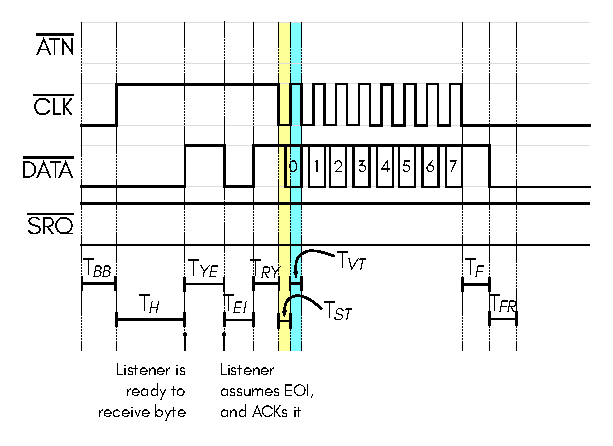
\includegraphics{images/IEC-Timing-Diagrams/IEC-Timing-Diagram-Send-Byte-EOI}
\end{center}

\begin{center}
    \setlength{\def\arraystretch{1.5}\tabcolsep}{6pt}
    \begin{longtable}{|L{0.6cm}|c|c|c|c|L{6cm}|}
      \hline
        \multicolumn{2}{|c|}{\textbf{Symbol}} & \textbf{Min} & \textbf{4541} & \textbf{Max} & \textbf{Description} \\
        \hline
        \endhead
        \multicolumn{2}{|c|}{T\textsubscript{BB}} & 100 & 100 & $\infty$ &
        Time between bytes. Talkers must wait long enough to allow the
        listener to register the end of the transmission of the
        previous byte, before the next byte can be sent. \\
        \hline
        \multicolumn{2}{|c|}{T\textsubscript{H}} & -- & N/A & $\infty$ & Listener
        hold-off. {\em Listener can hold of for any desired period of
          time, or for no time at all.} \\
        \hline
        \multicolumn{2}{|c|}{T\textsubscript{YE}} & 200 & 250 & $\infty$ &
        EOI indication delay.  The sender must wait at least 200
        microseconds for the receiver to recognise that a byte is
        being sent with EOI. If the delay is less than this, the
        receiver will not acknowledge the EOI. \\
        \hline
        \multicolumn{2}{|c|}{T\textsubscript{EI}} & 60 & 80 & $\infty$ &
        EOI acknowledge hold time. The receiver must pull the DATA
        line to 0V again for at least 60 microseconds, to allow the
        sender to detect this EOI acknowledgement pulse. \\
        \hline
        \multicolumn{2}{|c|}{T\textsubscript{RY}} & 60 & 80 & 100 &
        The talker response limit is a relatively narrow time window
        during which the talker must commence transmission of the
        byte. If it is too early, the listener may become
        desynchronised, because it has not hat time to prepare for
        reception after sending the EOI acknowledgement. If it is too
        long, the receiver may conclude the talker has stopped
        talking. \\
        \hline
        \multicolumn{2}{|c|}{T\textsubscript{ST}} & 20*  & 35 & $\infty$ &
        Data bit setup time. {\em Referred to as T\textsubscript{S} in
          the C64 Programmer's Reference Guide.}\\
        \hline
        \multicolumn{2}{|c|}{T\textsubscript{VT}} & 20*  & 35 & $\infty$ &
        Data bit valid hold time. {\em Referred to as
          T\textsubscript{V} in the C64 Programmer's Reference Guide.} \\
        \hline
        \multicolumn{2}{|c|}{T\textsubscript{F}} & --  & 1000 & 1000 &
        Frame handshake (acknowledge) timeout. \\
        \hline
        \multicolumn{2}{|c|}{T\textsubscript{FR}} & 0/60\^ & 0 & $\infty$ &
        EOI Frame acknowledge. The listener pulls DATA to 0V after a
        short period of time to acknowledge the byte sent with EOI. \\
        \hline
        \multicolumn{6}{l}{\em All time units are in micro seconds, unless
          otherwise indicated.} \\
        \multicolumn{6}{Y{10cm}}{* T\textsubscript{ST} is
          provided by the peripheral, not the controller. The 4541 is
          able to respond much faster than a C64 to serial bus events,
          and thus requires only 4 microsecond to ensure the CLK line has
          time to rise to 5V. 
          For controllers using software
          implementations of the protocol, such as the C64, the
          minimum is 80 microsecond.
          Therefore peripherals should always use
          a value of at least 80 microsecond for T\textsubscript{DA}.
        } \\
        \multicolumn{6}{Y{10cm}}{\^{} The
          Commodore{\texttrademark} 64 Programmer's Reference Guide
          lists 
          T\textsubscript{FR} as having a minimum duration of 60 microsecond.
          We see no evidence that 
          would suggest that any implementation requires a delay
          before the DATA line can be pulled low by the listener to
          acknowledge receipt of a byte.
        }
          \\
    \end{longtable}
\end{center}

\subsection{Receive Byte}

Receiving bytes on the IEC bus occurs identically to the sending
case.  The key difference is that the 4541 is tolerant of a much wider
range of timing parameters than software implementations of the bus
protocol. The 4541 requires not more than 4 microseconds for any
given bus state, which is the time required for the pull-up resistors
on the bus to allow lines to float back to 5V.  Internally, the 4541
is capable of detecting bit times shorter than 1 microsecond.

\section{Optional Integrated Data-Logger}

The 4541 is available in a variant that contains an embedded serial
peripheral bus data-logger. This is designed to aid with debugging
protocol errors on this bus. It commences capturing data whenever
command \$D0 is issued to the 4541, and
will capture data for approximately 4 milliseconds.

\begin{itemize}
  \item {\bf DATALOG0} The low-byte of the optional integrated serial
    peripheral bus data logger.  Writing \$00 to this register causes
    the read pointer to the data log to be reset to the beginning of
    the capture. Writing \$01 to this register, causes the
    read point of the data logger to be advanced by one time step.
    The time steps are approximately 1 microsecond, with additional
    time steps added whenever one of the signals on the serial
    peripheral bus changes state.
    \item {\bf DATALOG1} The high-byte of the optional integrated serial
      peripheral bus data logger. Different fields can be read at this
      address by writing the following values to the DATALOG0
      register:
      \begin{itemize}
        \item \$02 - Read low byte of IEC controller state machine
          state number.
        \item \$03 - Read high byte of IEC controller state machine
          state number.
        \item \$04 - Read low byte of number of cycles the previous bus state
          was held for.
        \item \$05 - Read high byte of number of cycles the previous bus state
          was held for.
        \end{itemize}
\end{itemize}

Each time-step records 16 bits of information about the serial
peripheral bus:
\begin{itemize}
\item {\bf DATALOG0 Bit 0} DATA line input value
\item {\bf DATALOG0 Bit 1} CLK line input value
\item {\bf DATALOG0 Bit 2} SRQ line input value
\item {\bf DATALOG0 Bit 3} DATA line output state
\item {\bf DATALOG0 Bit 4} CLK line output state
\item {\bf DATALOG0 Bit 5} SRQ line output state
\item {\bf DATALOG0 Bit 6} ATN line output state
\item {\bf DATALOG0 Bit 7} RESET line output state
\item {\bf DATALOG1} Access to the additional data logger fields.
\end{itemize}

The input values are the voltages that the 4541 reads on the
respective pins.  Separately, the data-logger records whether the 4541
is pulling each of those lines low.  This allows determination as to
whether a connected peripheral or the 4541 is pulling a given signal
low. This provides much more information than simply probing the lines
of the serial peripheral bus, where you cannot readily determine who
has pulled a given line low.

The following truth table explains how to interpret these signals:

\begin{center}
    \setlength{\def\arraystretch{1.5}\tabcolsep}{6pt}
    \begin{longtable}{|c|c|L{8cm}|}
        \hline
        \textbf{Input Value} & \textbf{Output Value} &
        \textbf{Meaning}  \\
        \hline
        \endhead
        1 & 1 & Signal is floating at 5V. No device is pulling it
        low. \\
        \hline
        0 & 1 & Signal is at 0V. The 4541 is not pulling it low,
        either a connected peripheral or the CIA is pulling it low. \\
        \hline
        0 & 0 & Signal is 0V. The 4541 is pulling it low. Other
        devices might also be pulling it low, but it's not possible to
        discriminate between these two situations.
        low. \\
        \hline
        1 & 0 & Signal is floating at 5V, but the 4541 is pulling it
        to 0V. Your computer is probably broken, or someone has
        connected 5V to the signal without a current-limiting
        resistor in between, in which case, your computer is about to be broken. \\
        \hline
    \end{longtable}
\end{center}

\subsection{Extracting Data from the Data Logger}

The following program extracts and displays the contents of the Data Logger as a
PETSCII waveform, like the one shown here:

\begin{center}
  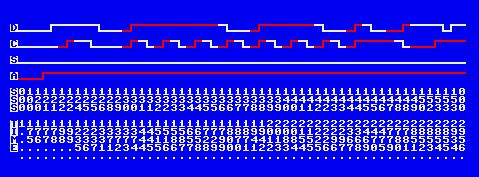
\includegraphics[width=0.7\linewidth]{images/IEC-Timing-Diagrams/iec-waveform-cropped}
\end{center}


% Program is too long to fit on a single page
\input{examples/iec-data-logger}
\input{examples/iec-data-logger-2}
